\documentclass{beamer}
\usetheme{Madrid}
\usepackage[utf8]{inputenc}
\usepackage[russian]{babel}
\usepackage{amsmath}
\usepackage{graphicx}

\title{Автоматическое выделение доменных границ в белках по пространственной структуре}
\author{ФИО, научный руководитель}
\date{2025}

\begin{document}

% Слайд 1: Титульный
\begin{frame}
  \titlepage
\end{frame}

% Слайд 2: Введение
\begin{frame}{Введение}
  \begin{itemize}
    \item Белковые домены — структурные и функциональные единицы белка
    \item Автоматическое определение границ доменов важно для аннотации и анализа белков
    \item Цель: разработать и сравнить методы выделения доменных границ по 3D-структуре
  \end{itemize}
\end{frame}

% Слайд 3: Формальная постановка задачи
\begin{frame}{Формальная постановка задачи}
  \begin{itemize}
    \item Дано: 3D-структура белка (PDB), последовательность остатков $R = (r_1, \ldots, r_n)$
    \item Требуется: построить бинарную маску $y \in \{0,1\}^n$, где $y_i=1$ — граница домена
    \item Модель: $f(\mathbf{X}, G) \to \hat{y}$, где $\mathbf{X}$ — признаки остатков, $G$ — граф контактов
  \end{itemize}
  \vspace{0.5em}
  \textbf{Задача:} $\arg\max_f \; \mathbb{E}_{(\mathbf{X}, G, y)} \; Q(f(\mathbf{X}, G), y)$
\end{frame}

% Слайд 4: Метрики качества
\begin{frame}{Метрики качества}
  \begin{itemize}
    \item IoU (границы): $\frac{|\hat{y} \cap y|}{|\hat{y} \cup y|}$
    \item IoU (домены): среднее IoU по сегментам
    \item Boundary F1-score: F1 по найденным границам с допуском
    \item Mean Boundary Deviation (MBD): среднее отклонение границ
  \end{itemize}
\end{frame}

% Слайд 5: Датасет и подготовка данных
\begin{frame}{Датасет и подготовка данных}
  \begin{itemize}
    \item SCOP: аннотированные домены, загрузка PDB-структур
    \item Формирование ground truth: маска границ по SCOP
    \item Train/test split, кросс-валидация
  \end{itemize}
\end{frame}

% Слайд 6: Классические методы (DOMAK, SPLIT)
\begin{frame}{Классические методы}
  \textbf{DOMAK:}
  \begin{itemize}
    \item Границы определяются по разрывам: $d_{i,i+1} = \|\mathbf{x}_{i+1} - \mathbf{x}_i\|$
    \item Если $d_{i,i+1} > t$, то $i$ — граница домена
    \item $t$ — эмпирический порог (обычно 8\AA)
    \item См. \textit{Siddiqui, A. S., Barton, G. J. (1995). Continuous and discontinuous domains: an algorithm for the automatic generation of reliable protein domain definitions. Protein Science, 4(5), 872-884.}
  \end{itemize}
  \vspace{0.5em}
  \textbf{SPLIT:}
  \begin{itemize}
    \item Пусть $k$ — число доменов (из разметки)
    \item Границы: $b_j = \left\lfloor \frac{j \cdot n}{k} \right\rfloor,\; j=1,\ldots,k-1$
    \item Каждый сегмент $[b_{j-1}, b_j)$ — домен
    \item Простой baseline, не учитывает структуру
  \end{itemize}
  \vspace{0.5em}
  \textbf{Ссылки:}
  \begin{itemize}
    \item \footnotesize Siddiqui, A. S., Barton, G. J. (1995). Protein Science, 4(5), 872-884.
    \item \footnotesize Holland, T. A., Veretnik, S., Shindyalov, I. N., Bourne, P. E. (2006). Protein domain identification: a structural biology perspective. Structure, 14(7), 997-1006.
  \end{itemize}
\end{frame}

% Слайд 7: GCN-модель (DomainGCN)
\begin{frame}{GCN-модель (DomainGCN)}
  \begin{itemize}
    \item Вход: $\mathbf{X} \in \mathbb{R}^{n \times 3}$ — координаты CA, $G=(V,E)$ — граф контактов
    \item Граф: $A_{ij} = 1$ если $\|\mathbf{x}_i - \mathbf{x}_j\| < 8\AA$
    \item Модель: $\mathbf{H}^{(l+1)} = \sigma(\tilde{D}^{-1/2} \tilde{A} \tilde{D}^{-1/2} \mathbf{H}^{(l)} W^{(l)})$
    \item 4 слоя GCNConv, выход — вероятности классов для каждого остатка
    \item Функция потерь: $\mathcal{L} = -\sum_i w_{y_i} \log p_{i, y_i}$, $w_1 \gg w_0$
  \end{itemize}
  \vspace{0.5em}
  \textbf{Ссылки:}
  \begin{itemize}
    \item \footnotesize Kipf, T. N., Welling, M. (2017). Semi-Supervised Classification with Graph Convolutional Networks. ICLR.
    \item \footnotesize Gainza, P. et al. (2020). Deciphering interaction fingerprints from protein molecular surfaces using geometric deep learning. Nature Methods, 17(2), 184-192.
  \end{itemize}
\end{frame}

% Слайд 8: Постановка эксперимента
\begin{frame}{Постановка эксперимента}
  \begin{itemize}
    \item Обучение на train, оценка на test
    \item Сравнение с DOMAK и SPLIT по всем метрикам
    \item Кросс-валидация для оценки дисперсии
  \end{itemize}
\end{frame}

% Слайд 9: Результаты (таблица)
\begin{frame}{Результаты сравнения}
  \begin{center}
    \includegraphics[width=0.95\textwidth]{results_metrics.png} % вставьте скриншот/таблицу
  \end{center}
  \begin{itemize}
    \item GCN превосходит классические методы по большинству метрик
  \end{itemize}
\end{frame}

% Слайд 10: Примеры предсказаний
\begin{frame}{Примеры предсказаний}
  \begin{itemize}
    \item Визуализация: истинные и предсказанные границы на белке
    \item Ошибки: ложные/пропущенные границы
  \end{itemize}
  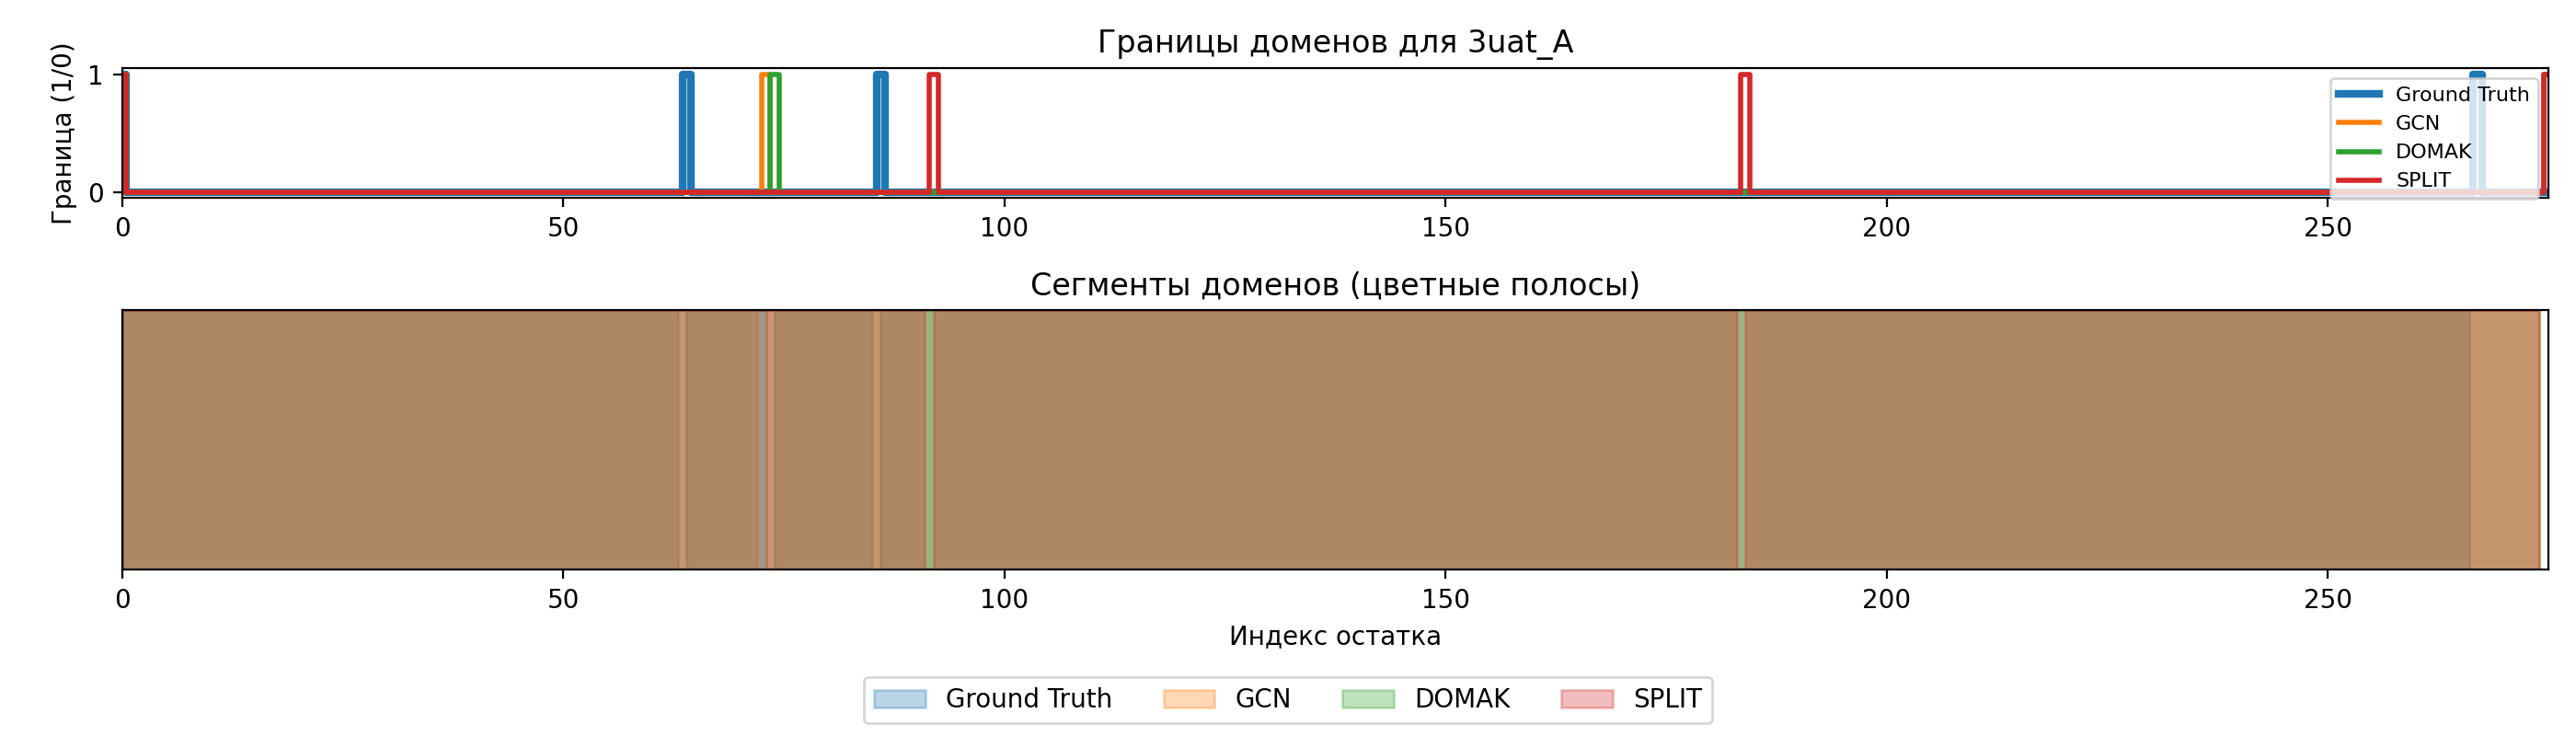
\includegraphics[width=0.8\textwidth]{example_pred.png} % вставьте пример
\end{frame}

% Слайд 11: Выводы
\begin{frame}{Выводы}
  \begin{itemize}
    \item GCN-модель успешно выделяет границы доменов по структуре
    \item Классические методы уступают по точности
    \item Возможности для улучшения: дополнительные признаки, архитектуры
  \end{itemize}
\end{frame}

% Слайд 12: Спасибо за внимание
\begin{frame}{Спасибо за внимание!}
  \begin{center}
    Вопросы?
  \end{center}
\end{frame}

\end{document}
